\documentclass[notes.tex]{subfiles}
\begin{document}

\chapter{Resultados experimentais}

A implementação do algoritmo descrito foi feita na linguagem python 3.8.
A partir disso, foram executados os testes para avaliar a presença das propriedades desejadas no modelo.
Para os testes iniciais, foram utilizados valores descritos no \autoref{qua:base_params}.

\begin{quadro}[htbp]
    \centering
    \caption{Parâmetros básicos}
    \label{qua:base_params}
    \begin{tblr}{|r|r|r|r|r|r|r|r|} \hline
        \SetCell{c} $N$ & \SetCell{c} $E_\text{wth}^\text{max}$ & \SetCell{c} $E_\text{btw}^\text{max}$ & \SetCell{c} $MTE$ & \SetCell{c} $\A$ & \SetCell{c} $K$ & \SetCell{c} $\theta$ & \SetCell{c} $\text{NbRep}$ \\ \hline
         1000 & 45 & 3 & 7000 & (1, 1) & (6, 2) & $\sfrac{1}{10}$ & 20 \\ \hline
    \end{tblr}
    \fonte{elaborado pelo autor.}
\end{quadro}

\section{Presença de comunidades}

A presença de comunidades como uma propriedade de redes complexas está tipicamente atrelada a ideia de haverem mais arestas internas a uma comunidade do que arestas que atravessem a fronteira entre duas comunidades.
Esse entendimento é solidificado na função de modularidade $Q$ de \citeonline{girvan2002community}, conforme descrito na equação \ref{eq:mod}.
\citeonline{shen2009detect} descrevem uma adaptação, modularidade estendida $EQ$, para a aplicação em coberturas (em oposição a partições), conforme equação \ref{eq:mod_e}.
Essa aplicação em coberturas destaca a possibilidade de comunidades sobrepostas.
A aplicação de $EQ$ recursivamente, de forma a considerar o subgrafo com os membros da comunidade dividido entre as comunidades que a compõe descreve a propriedade de comunidades hierárquicas.

\begin{equation}
O_i = \left[\sum_{c \in C_n| L_{c} = i-1}V_c\right] - \left[\sum_{c \in C_n| L_{c} = i}V_c\right]
\end{equation}

A presença de sobreposição nas comunidades pode ser medida como um função $O_i$ que calcula a quantidade de vértices presentes em mais de uma comunidade de nível $i$.
O valor é dado pela diferença da quantidade de vértices em comunidades de nível $i$ e a quantidade de vértices em comunidades de nível $i+1$.
O efeito disso é que vértices que estejam em duas comunidades distintas de nível $i+1$ ou menores, serão contados duas vezes, mas os que pertencem a duas comunidades de nível $i$ ou menores serão compensadas.
Por fim, a soma de $O_i$ para todos os níveis será anotada como  $O$.

Observa-se na \autoref{tab:mod_base_params} os valores de $EQ$ para 10 execuções do modelo com os parâmetros básicos ($B_0$ a $B_9$).
Para as comunidades de primeiro nível, isso é, as que são compostas por sub-comunidades, a função gera uma média de aproximadamente 0,8, que indica uma estrutura de comunidade muito expressiva.
No segundo nível, o valor médio foi de aproximadamente 0,6 indicando comunidades menos expressivas mas ainda presentes.

\begin{table}[htbp]
    \centering
    \caption{Modularidade com os parâmetros básicos}
    \label{tab:mod_base_params}
    \begin{tblr}{l|r|r|r|r} \hline
        \SetCell{c} Execução & \SetCell{c} $EQ_1$ & \SetCell{c} $EQ_2$  & \SetCell{c} $O_1$ & \SetCell{c} $O_2$\\ \hline
        $B_0$ & 0,71695 & 0,79204 & 16 & 235 \\ \hline
        $B_1$ & 0,72441 & 0,79760 & 18 & 211 \\ \hline
        $B_2$ & 0,70039 & 0,79391 & 14 & 252 \\ \hline
        $B_3$ & 0,73633 & 0,79622 & 13 & 190 \\ \hline
        $B_4$ & 0,71758 & 0,78549 & 26 & 235 \\ \hline
        $B_5$ & 0,73179 & 0,79201 & 33 & 224 \\ \hline
        $B_6$ & 0,74779 & 0,79828 & 15 & 213 \\ \hline
        $B_7$ & 0,73912 & 0,80411 & 20 & 200 \\ \hline
        $B_8$ & 0,74237 & 0,80504 & 19 & 194 \\ \hline
        $B_9$ & 0,71339 & 0,79877 & 17 & 237 \\ \hline
        Média & 0,73701 & 0,79635 & 19 & 219 \\ \hline
    \end{tblr}
    \fonte{elaborado pelo autor.}
\end{table}

A \autoref{tab:mod_base_params} indica também os valores de sobreposição entre comunidades de primeiro ($O_1$) e segundo nível ($O_2$).
Os valores indicam quem em média, dos mil vértices presentes em um grafo como o observado, dezessete estarão em duas comunidades de primeiro nível e em média duzentos e vinte e cinto vértices estarão em duas comunidades de segundo nível.
O que esses valores indicam é que até vinte e quatro por cento dos vértices, para essa parametrização, estariam distribuídos em mais de uma comunidade.

Naturalmente, a escolha de valores distintos para os parâmetros pode ser feita para reforçar as características desejáveis.
Limitando o valor de $MTE$ e considerando uma estrutura de comunidades gerada com  $K = (9, 2, 2, 2)$, obteve-se os dados distritos na \autoref{tab:mod_pro_params}.
Observa-se que a redução do número mínimo foi feita para evitar a descaracterização das comunidades folha, considerando que o valor de $K$ gera 72 dessas.

\begin{table}[htbp]
    \centering
    \caption{Modularidade com $K = (9, 2, 2, 2)$}
    \label{tab:mod_pro_params}
    \begin{tblr}{l|r|r|r|r|r} \hline
        \SetCell{c} Execução & \SetCell{c} $EQ_1$ & \SetCell{c} $EQ_2$ & \SetCell{c} $EQ_3$ & \SetCell{c} $EQ_4$ & \SetCell{c} $O$ \\ \hline
        $M_0$ & 0,96702 & 0,95833 & 0,93128 & 0,87673 & 0 \\ \hline
        $M_1$ & 0,96721 & 0,95979 & 0,93388 & 0,88221 & 0 \\ \hline
        $M_2$ & 0,96514 & 0,95933 & 0,93357 & 0,87722 & 0 \\ \hline
        $M_3$ & 0,96541 & 0,95711 & 0,92974 & 0,87888 & 0 \\ \hline
        $M_4$ & 0,96672 & 0,95868 & 0,93582 & 0,88090 & 0 \\ \hline
        Média & 0,96630 & 0,95865 & 0,93286 & 0,87919 & 0 \\ \hline
    \end{tblr}
    \fonte{elaborado pelo autor.}
\end{table}

O incremento nos valores obtidos é atribuível à existência de mais comunidades para as quais distribuir os vértices, não apenas em profundidade mas também em diâmetro.
Descartando-se a possibilidade de ser a alteração do valor de $MTE$ ao realizar testes com este zerado mas mantendo o $K$ padrão.
Em compensação, essa parametrização faz com que a escolha de comunidades folha se torne muito mais provável, anulando a possibilidade de comunidades sobrepostas.
Esse comportamento ocorre pois no processo de escolha das comunidades a ordenação das comunidades ocorre preferindo comunidades que têm os representantes mais próximos, e as comunidades folha por serem em maior quantidade são muito mais prováveis de serem escolhidas.

Nos testes descritos na \autoref{tab:mod_var_params}, onde com $MTE = 0$ realizou-se uma exploração dos valores de $EQ$ para diversos valores em $K$.
Note-se o caso $M_9$ como contra exemplo do impacto de $K$ na modularidade, bem como o exemplo $M_6$, que nas comunidades de primeiro tem $EQ = 0,5$.

\begin{table}[htbp]
    \centering
    \caption{Modularidade com variação de $K$}
    \label{tab:mod_var_params}
    \begin{tblr}{l|r|r} \hline
        \SetCell{c} Execução & $K$ & \SetCell{c} Média de $EQ$ \\ \hline
        % (0.59322 +0.94915 +0.79429)/3 = 0.778887
        $M_5$ & $(5, 5, 5)$ & 0,77889 \\ \hline 
        %(0.96943 +0.86339 +0.49881)/3 = 0.77721
        $M_6$ & $(2, 4, 8)$ & 0,77721 \\ \hline
        % (0.96947 +0.93266 +0.87089)/3 = 0.92434
        $M_7$ & $(8, 2, 4)$ & 0,92434 \\ \hline
        $M_8$ & $(100)$ & 0,95152 \\ \hline
        $M_9$ & $(3)$ & 0,49024 \\ \hline
    \end{tblr}
    \fonte{elaborado pelo autor.}
\end{table}

Alternativamente, é possível modificar significativamente os valores obtidos para a modularidade com os parâmetros $E_\text{btw}^\text{max}$ e $E_\text{wth}^\text{max}$.
% (0.48115 + 0.4421)/2 = 0.461625
Na execução $M_{10}$ utilizou-se os demais parâmetros nos valores padrão, mas com $E_\text{btw}^\text{max}=45$ e $K = (2, 2)$, para um $EQ$ médio de 0,46.

\section{Homofilia e Homogeneidade}

Homogeneidade é a principal propriedade das comunidades definidas por semelhança de vértices, ela está intimamente ligada à propriedade de homofilia.
Assumindo a distância euclideana como função de semelhança, a forma natural de medir a homogeneidade das comunidades descritas por uma cobertura é a inércia e a razão da inércia entre diferentes níveis de comunidades.

\subsection{Inércia}

Inércia, definida como a soma dos quadrados das distâncias de cada membro de um conjunto com a média do conjunto, sumariza quão semelhantes ou dissemelhantes os membros são.
A razão entre a inércia em diferentes níveis é facilmente extrapolada do conceito de razão de inércia introduzido por \citeonline{largeron2015generating}.
Assumindo que as comunidades de uma rede complexa sejam homogêneas e hierárquicas, é natural que as comunidades mais específicas (sub-comunidades), tenham menos diversidade que as comunidade mais generalistas.
Tendo em vista que a inércia calculada com uma cobertura deve levar em conta que vértices serão contados múltiplas vezes se estiverem presentes em múltiplas comunidades, a inércia para um nível $l$ segue descrita na equação \ref{eq:inercia_l}.
Considerando que $C_l$ é o conjunto de comunidades de nível  $l$.

\begin{equation}\label{eq:inercia_l}
    I_l = \sum_{c \in C_l}\frac{\sum_{v \in c} |v-g_c|^2}{|c|}
\end{equation}

$I_l$ apresenta uma forma de comparação entre diferentes coberturas, de forma a identificar qual seria mais homogênea dado um mesmo conjunto do vértices.
A extensão do conceito de inércia para a razão entre a inércia aplicada a dois níveis distintos se dá para isolar o fator de escala.
Isso é, $\sfrac{I_l}{I_0}$ descreve não apenas quão homogêneo são os agrupamentos estabelecidos, mas o quão homogêneos eles são em relação à população em geral.
Note-se que $I_0$ nesse contexto se refere à comunidade $C_n$, isso é, a comunidade que contém todos os vértices.

\subsection{Distância esperada}

A homofilia, como propriedade de redes complexas onde os vértices tendem a estarem adjacentes à vértices semelhantes.
Em um sistema com atributos discretos, é facilmente estabelecido uma função $\Delta$  que descreve o quão semelhantes os vértices adjacentes são do que seria esperado em um modelo nulo.
O modelo nulo trivial neste caso é a consideração de vértices conectados com igual probabilidade, mantendo-se a mesma quantidade de vértices e arestas, conforme descrito por \citeonline{easley2010networks}.

A adaptação para um modelo de um espaço contínuo de múltiplas dimensões se dá calculando uma aproximação da distância média entre cada par de vértices, essa média, $H_e$, é o valor que seria esperado se o grafo não fosse homofílico.
O valor real é calculado como a média da distância dos pontos adjacentes, $H_r$.

\subsection{Resultados}

Na \autoref{tab:iner_base_params} estão discriminados os valores médios de inércia para as comunidades organizadas por nível.
A leitura que se pode fazer desses dados, em especial das médias, é: em média uma comunidade de primeiro nível tem 38\% da diversidade que se encontra na população geral; e em média uma comunidade de segundo nível (sub-comunidade) tem 33\% da diversidade presente na população em geral.
Por fim, em média a distância entre dos vértices adjacentes é metade do que seria esperado sem a homofilia, indicando a presença dessa propriedade.

\begin{table}[htbp]
    \centering
    \caption{Homogeneidade e homofilia com os parâmetros básicos}
    \label{tab:iner_base_params}
    \begin{tblr}{l|r|r|r|r} \hline
        \SetCell{c} Execução & \SetCell{c} $\sfrac{I_1}{I_0}$ & \SetCell{c} $\sfrac{I_2}{I_0}$ & \SetCell{c} $\sfrac{I_1+I_2}{2I_0}$ & \SetCell{c} $\sfrac{H_r}{H_e}$
        \\ \hline
$B_0$ & 0,38193 & 0,34155 & 0,36174 & 0,45942 \\ \hline
$B_1$ & 0,34067 & 0,30168 & 0,32118 & 0,45920 \\ \hline
$B_2$ & 0,34262 & 0,29697 & 0,31980 & 0,49265 \\ \hline
$B_3$ & 0,35961 & 0,29986 & 0,32974 & 0,48305 \\ \hline
$B_4$ & 0,41670 & 0,37592 & 0,39631 & 0,52725 \\ \hline
$B_5$ & 0,35321 & 0,28246 & 0,31784 & 0,46047 \\ \hline
$B_6$ & 0,37795 & 0,29310 & 0,33553 & 0,46127 \\ \hline
$B_7$ & 0,35209 & 0,29903 & 0,32556 & 0,45348 \\ \hline
$B_8$ & 0,36251 & 0,32820 & 0,34536 & 0,46364 \\ \hline
$B_9$ & 0,36874 & 0,32936 & 0,34905 & 0,50499 \\ \hline
Média & 0,36560 & 0,31481 & 0,34021 & 0,47654 \\ \hline
    \end{tblr}
    \fonte{elaborado pelo autor.}
\end{table}

Naturalmente, existe uma influência significativa que a quantidade de comunidades tem neste valor.
Observe-se na \autoref{tab:iner_pro_params}, com mais comunidades para distribuir os vértices, as comunidades ficam significativamente mais homogêneas.
Como efeito disso, a distância entre vértices conectados é bastante reduzida.

\begin{table}[htbp]
    \centering
    \caption{Homofilia e Homogeneidade com $K = (9, 2, 2, 2)$}
    \label{tab:iner_pro_params}
    \begin{tblr}{l|r|r|r|r|r} \hline
        \SetCell{c} Execução & \SetCell{c} $\sfrac{I_1}{I_0}$ & \SetCell{c} $\sfrac{I_2}{I_0}$ & \SetCell{c} $\sfrac{I_3}{I_0}$ & \SetCell{c} $\sfrac{I_4}{I_0}$ & \SetCell{c} $\sfrac{H_r}{H_e}$ \\ \hline
        $M_0$ & 0,18740 & 0,11020 & 0,05650 & 0,03240 & 0,15975 \\ \hline
        $M_1$ & 0,18766 & 0,11563 & 0,06017 & 0,03277 & 0,16491 \\ \hline
        $M_2$ & 0,18446 & 0,11812 & 0,05993 & 0,03526 & 0,17281 \\ \hline
        $M_3$ & 0,18566 & 0,11307 & 0,06003 & 0,03169 & 0,16211 \\ \hline
        $M_4$ & 0,18111 & 0,11163 & 0,05563 & 0,03016 & 0,16158 \\ \hline
        Média & 0,18526 & 0,11373 & 0,05845 & 0,03246 & 0,16423 \\ \hline
    \end{tblr}
\fonte{elaborado pelo autor.}
\end{table}

% (0.18740 + 0.18766 + 0.18446 + 0.18566 + 0.18111)/5 = 0.18526
% (0.11020 + 0.11563 + 0.11812 + 0.11307 + 0.11163)/5 = 0.11373
% (0.05650 + 0.06017 + 0.05993 + 0.06003 + 0.05563)/5 = 0.05845
% (0.03240 + 0.03277 + 0.03526 + 0.03169 + 0.03016)/5 = 0.03246
% (0.15975 + 0.16491 + 0.17281 + 0.16211 + 0.16158)/5 = 0.16423

Também de forma natural, existe uma relação entre o parâmetro $\theta$ e a inércia.
É apontado na \autoref{tab:iner_var_params} a variação da inércia conforme se altera $\theta$.
Duas características dos dados descritos são relevantes, primeiramente com $\theta = 1$ se as comunidades não estivessem sendo construídas ortogonalmente, seriam esperadas comunidades onde a diversidade interna se aproximaria da diversidade da população geral, mas não é isso o que se observa.
Isso é, em um modelo nulo, onde não existe correlação entre os atributos do vértice e a comunidade em que ele participa, seria esperado uma razão de inércia que tendesse a um.

\begin{table}[htbp]
    \centering
    \caption{Homofilia e Homogeneidade com $\theta$ variável}
    \label{tab:iner_var_params}
    \begin{tblr}{l|r|r|r|r} \hline
        \SetCell{c} Execução & \SetCell{c} $\theta$ & \SetCell{c} $\sfrac{I_1}{I_0}$ & \SetCell{c} $\sfrac{I_2}{I_0}$ &
        \SetCell{c} Média
        \\ \hline
        $I_0$ & \multirow{3}{*}{1,00} & 0,78255 & 0,73782 & \multirow{3}{*}{0,71637} \\ \hline
        $I_1$ &                       & 0,70558 & 0,67610 &                          \\ \hline
        $I_2$ &                       & 0,70773 & 0,68841 &                          \\ \hline
        $I_3$ & \multirow{3}{*}{0,66} & 0,40448 & 0,34173 & \multirow{3}{*}{0,36539} \\ \hline
        $I_4$ &                       & 0,40280 & 0,33749 &                          \\ \hline
        $I_5$ &                       & 0,37041 & 0,33541 &                          \\ \hline
        $I_6$ & \multirow{3}{*}{0,33} & 0,34582 & 0,29460 & \multirow{3}{*}{0,34005} \\ \hline
        $I_7$ &                       & 0,36632 & 0,30172 &                          \\ \hline
        $I_8$ &                       & 0,40126 & 0,33059 &                          \\ \hline
    \end{tblr}
\fonte{elaborado pelo autor.}
\end{table}


O segundo ponto a ser destacado é que $\theta$ não é um controle direto sobre a inércia, nos casos com  $\theta=0,66$, $\theta=0,33$ e $\theta=0,1$ (\autoref{tab:iner_base_params}), a razão se manteve em um mesmo patamar, entre 34\% e 40\%.
Existem outros fatores que afetam diretamente a homogeneidade das comunidades, e que são mais dificilmente controlados por parâmetros.

\section{Visualização}

Uma das características da propriedade de existência de comunidades é que a definição de comunidade é dependente de contexto.
Ainda assim, parece haver um entendimento natural de comunidades e de suas propriedades a partir da visualização das mesmas.
Segue a baixo a renderização dos grafos $B_0$ e $M_0$, gerados respectivamente com os parâmetros padrão e com os parâmetros otimizando para a modularidade (mais valores em $K$ e valores maiores).

A renderização desses grafos conta com uma codificação de forma que vértices que estejam na mesma comunidade de primeiro nível compartilhem o formato, e vértices que estejam na mesma comunidade de segundo nível compartilhem as cores, como é observável na \autoref{fig:m0}.
Vértices que estejam em mais de uma comunidade de segundo nível terão a cor branca, e vértices que estejam em mais de uma comunidade de primeiro nível terão o formato de círculo.
Dessa forma, é possível identificar as áreas de sobreposição, bem como os primeiros níveis da hierarquia de comunidades.

\begin{figure}[htpb]
    \centering
    \caption{$M_0$ renderizado aproximando os vértices adjacentes}\label{fig:m0}
    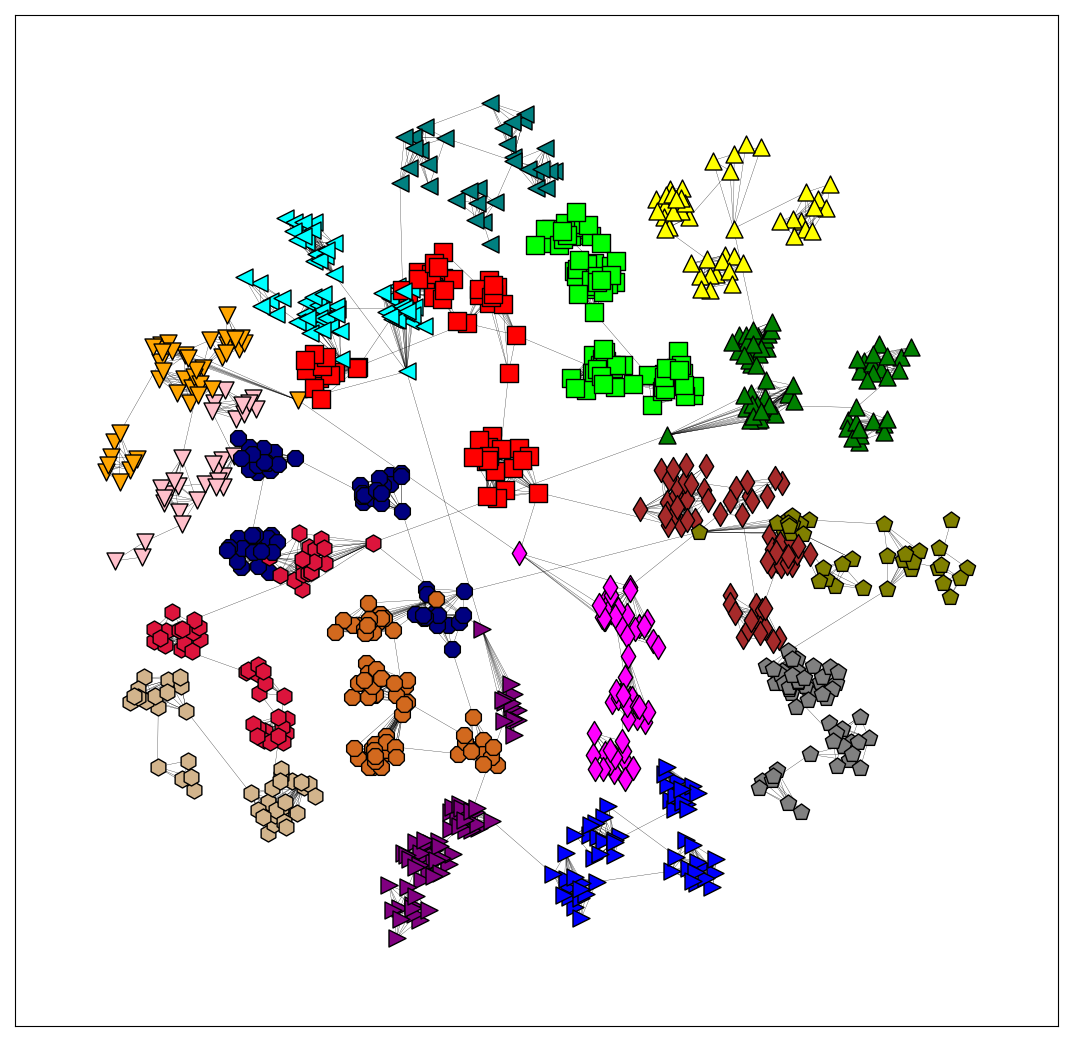
\includegraphics[width=\textwidth, height=0.6\textheight]{figures/m0.png}
    \fonte{elaborado pelo autor.}
\end{figure}

Na \autoref{fig:m0} está a renderização do grafo $M_0$ com o posicionamento dos vértices de forma a minimizar a distância deles na imagem.
Além das divisões entre comunidades que estão categorizadas com os formatos e com as cores, é visível uma divisão interna de pequenos grupos densamente conexos.
Essa visualização e entendimento intuitivo da divisão é decorrente de uma presença muito acentuada da propriedade de comunidades.

Essa divisão mais presenta, conforme já foi distrito anteriormente, é responsável também pela falta de vértices em regiões sobrepostas, de certa forma sacrificando ganhos nessa propriedade (sobreposição) para ganhar maior definição em outra (comunidades hierárquicas).
A \autoref{fig:m0_pos} e a \autoref{fig:m0_pos_wires} demonstram isso.
Ambas apresentam os vértices posicionados com base nos seus atributos, de forma que o centro (mais próximo a origem) e mais densamente povoado, no entanto a \autoref{fig:m0_pos_wires} não renderiza os vértices, apenas as arestas.
Com isso, é abundantemente claro o quão fortemente delineadas são as comunidades.
Demonstra-se que cada comunidade possui um domínio absoluto sobre alguma região do espaço onde os vértices se encontram.

\begin{figure}[htpb]
    \centering
    \caption{$M_0$ renderizado com os vértices posicionado pelos seus atributos}\label{fig:m0_pos}
    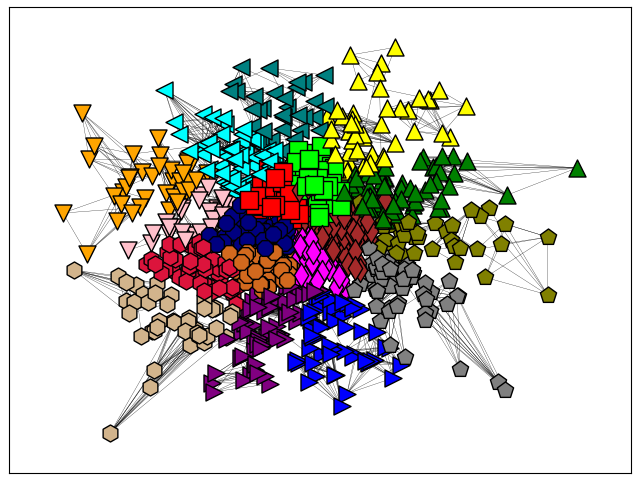
\includegraphics[width=0.8\textwidth, height=0.32\textheight]{figures/m0_pos.png}
    \fonte{elaborado pelo autor.}
\end{figure}

\begin{figure}[htpb]
    \centering
    \caption{$M_0$ renderizado com os vértices posicionado pelos seus atributos (apenas arestas)}\label{fig:m0_pos_wires}
    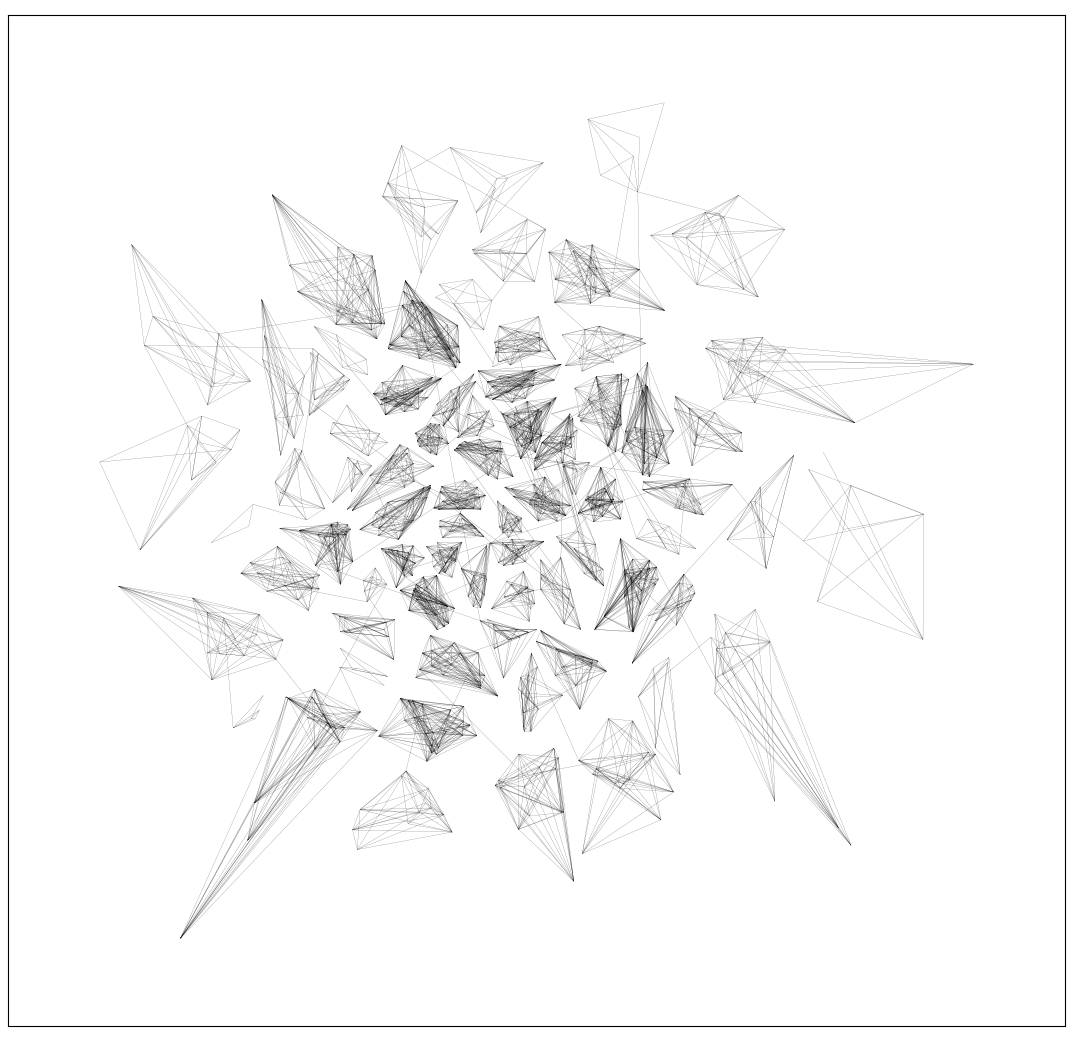
\includegraphics[width=\textwidth, height=0.52\textheight]{figures/m0_pos_wires.png}
    \fonte{elaborado pelo autor.} \end{figure}

A \autoref{fig:b0_pos} e a \autoref{fig:b0_pos_wires} fazem a mesma distinção, mas com o grafo $B_0$.
$B_0$ apresenta um conjunto de comunidades onde ocorre a sobreposição, não apenas no sentido de comunidades sobrepostas, mas em um sentido mais simples, de que há vértices que não pertencem a comunidade (e que não tem ligações com ela) ocupando o mesmo espaço.
Novamente, esse é um efeito de uma menor proporção de comunidades.

A visualização das arestas mostra uma divisão visual das comunidades, com uma comunidade no centro e cinco comunidades a rodeando.
Dessas seis comunidades, é possível identificar que existem grupos distintos dentro delas, isso é, as sub-comunidades são visíveis, mas pela natureza delas (e presença de vértices que pertencem as duas), são divisões muito menos precisas.

O mesmo grafo está exibido novamente na \autoref{fig:b0} e na \autoref{fig:b0_wires}.
Nelas é possível identificar mais claramente as áreas de sobreposição das comunidades de segundo nível (identificadas por não terem cor) bem como a presença de mais arestas internas as comunidades, naturalmente.

\begin{figure}[htpb]
    \centering
    \caption{$B_0$ renderizado com os vértices posicionado pelos seus atributos}\label{fig:b0_pos}
    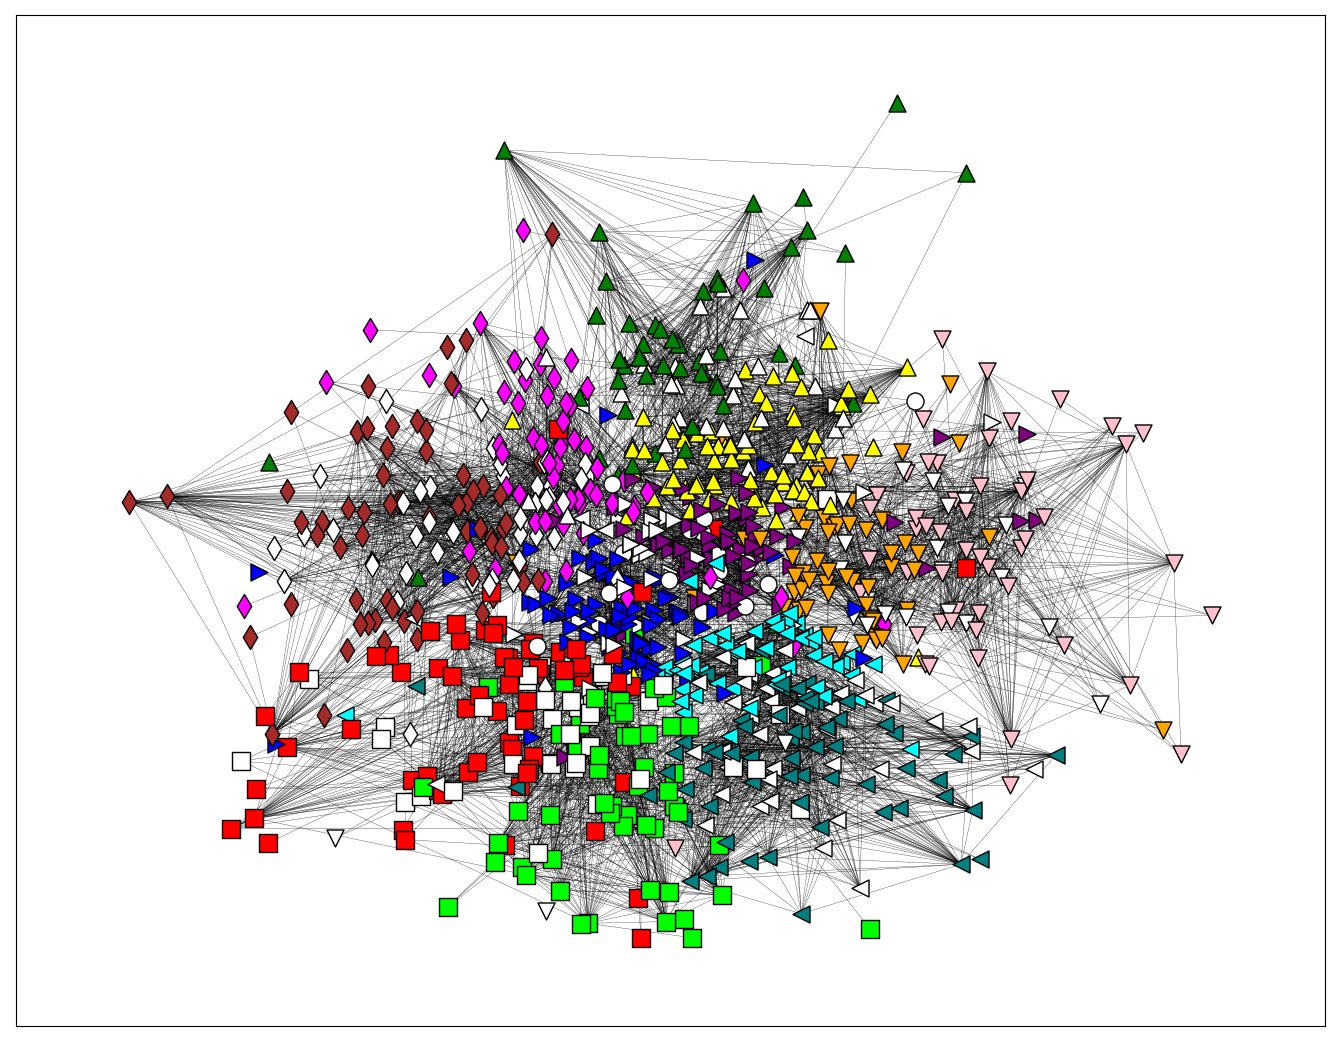
\includegraphics[width=\textwidth, height=0.52\textheight]{figures/b0_pos.png}
    \fonte{elaborado pelo autor.}
\end{figure}

\begin{figure}[htpb]
    \centering
    \caption{$B_0$ renderizado com os vértices posicionado pelos seus atributos (apenas arestas)}\label{fig:b0_pos_wires}
    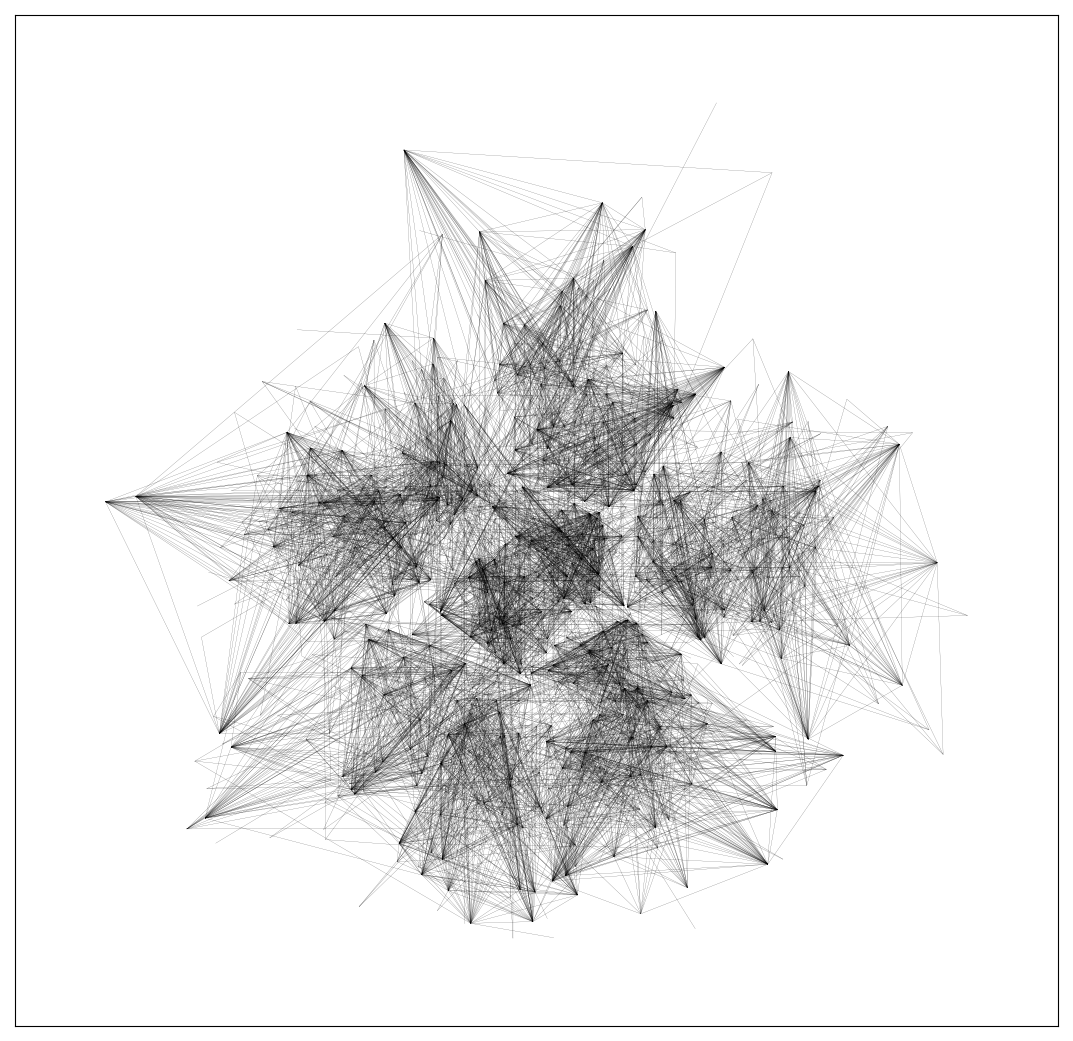
\includegraphics[width=0.8\textwidth, height=0.32\textheight]{figures/b0_pos_wires.png}
    \fonte{elaborado pelo autor.}
\end{figure}

\begin{figure}[htpb]
    \centering
    \caption{$B_0$ renderizado aproximando os vértices adjacentes}\label{fig:b0}
    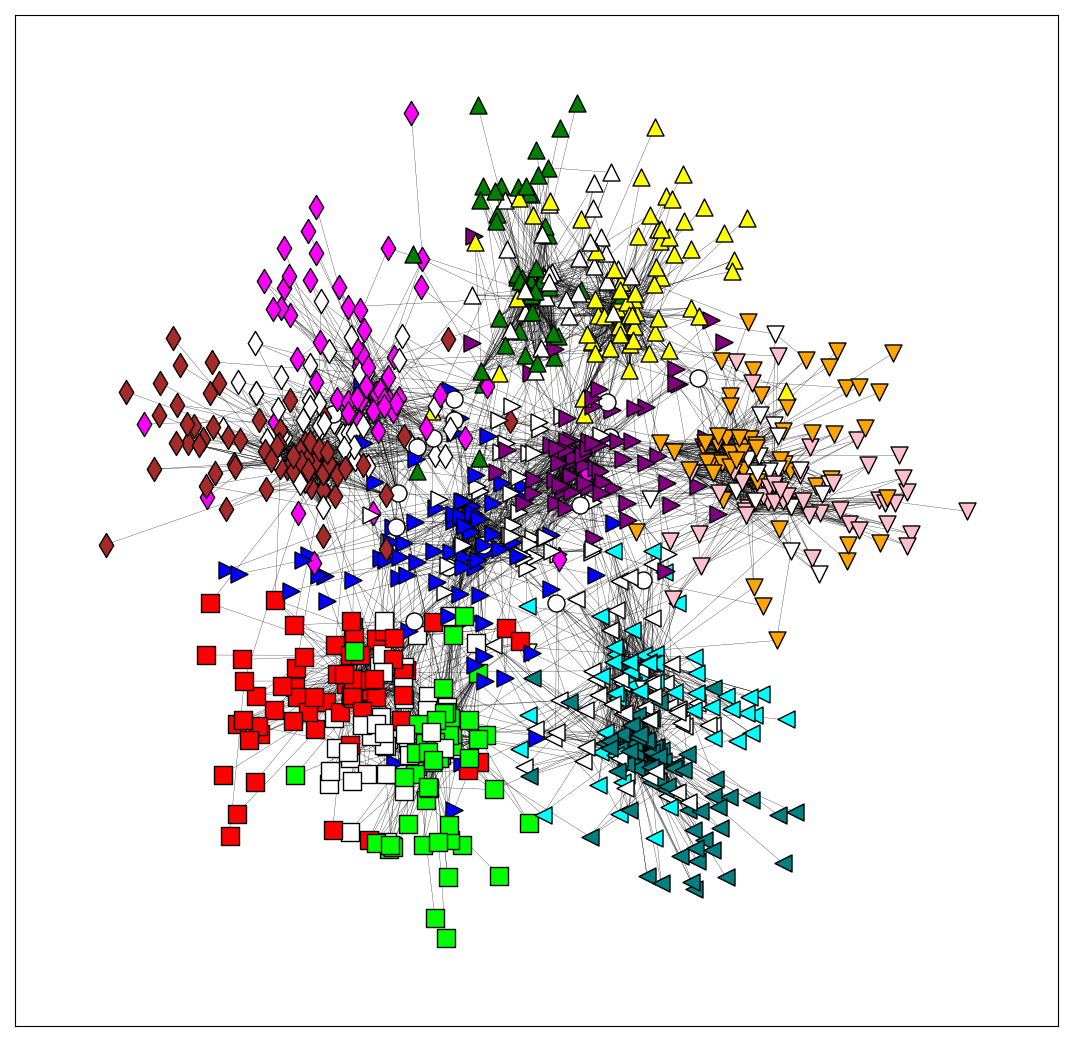
\includegraphics[width=\textwidth, height=0.42\textheight]{figures/b0.png}
    \fonte{elaborado pelo autor.}
\end{figure}

\begin{figure}[htpb]
    \centering
    \caption{$B_0$ renderizado aproximando os vértices adjacentes (apenas arestas)}\label{fig:b0_wires}
    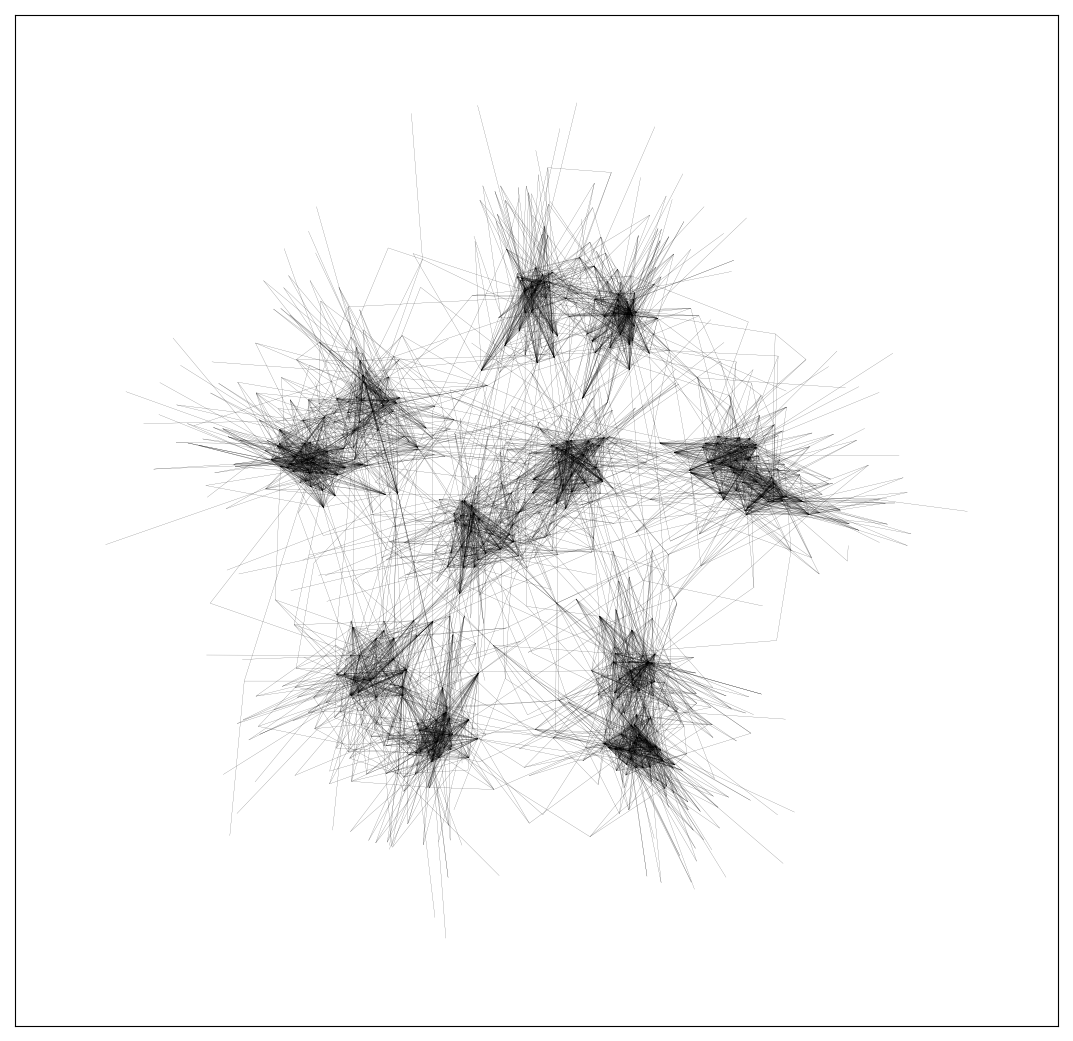
\includegraphics[width=1\textwidth, height=0.42\textheight]{figures/b0_wires.png}
    \fonte{elaborado pelo autor.}
\end{figure}

\end{document}
